\documentclass[runningheads]{llncs}

\usepackage{graphicx}
\usepackage{hyperref}
\usepackage[utf8]{inputenc}
\usepackage{enumerate}
\usepackage{amsmath}
\usepackage{bm}

\usepackage{xcolor}
\usepackage{listings}
\lstset{basicstyle=\ttfamily,
  showstringspaces=false,
  commentstyle=\color{gray},
  keywordstyle=\color{blue},
  breaklines=true
}

\renewcommand{\labelitemi}{$\bullet$}

\begin{document}

\title{Network Security in Practice}
\subtitle{Secrets Management}

\author{Johannes Kroschewski, Nils Straßenburg \\
Subervisors: Dr. Feng Cheng, David Jaeger}

\authorrunning{J. Kroschewski, N. Straßenburg}

\institute{Hasso-Plattner-Institut, Prof.-Dr.-Helmert-Str. 2–3, Germany 
\email{AUTHOR@student.hpi.de}}

\maketitle              

\begin{abstract}
Back in the day, applications were mainly deployed in a private environment secured with, e.g. firewalls and intrusion detection systems, but the inside of the network stayed completely soft. The move into the cloud has broken the assumption that the network perimeter is secure. Consequently, several questions arise from this architecture of extreme decentralization:

\begin{itemize}  
    \setlength\itemsep{1mm}
    \item How can a secret be distributed to its application?
    \item How can a secret be updated?
    \item How can a secret be revoked in case of a breach?
\end{itemize}

In this report, we discuss how these questions can be answered. As a first step, we give an introduction to the topic and define the term \textit{Secrets Management} and set a clear scope for this work. Afterwards, we first discuss some key concepts, and present a general security model for tools that help us to build a process for Secrets Management. In the following, we present and compare the basic architecture of the open source tool \textit{Vault} and the AWS solution for Secrets Management. Finally, we give some practical insights into the Secrets Management tool \textit{Vault}.

\end{abstract}

\newpage

\section{Security in a world of multiple clouds}

Security in the traditional private data center is oftentimes implemented following a perimeter-centric approach. To reduce the blast radius of the network, VLANs and software-defined networks are used to split the network into multiple pieces-each of which runs services corresponding to the line of business. All traffic is constrained over a central ingress and egress point that is used to deploy different types of middleware to secure the network e.g. firewalls, WAF, IDS. This approach makes a clean distinction into high- and low-trust Zones and asserts that any traffic that makes it through all appliances, policies, and checkpoints is privileged and trusted. 

Today, most companies apply a multi-cloud architecture and if not, are planning follow it \cite{ref_url_ibm}. As shown in \autoref{perimeter_cloud}, this means that applications are running in different regions and are connected to each other using direct peering relationships or VPNs. These applications are one API away from any node in these environments being able to receive or send traffic out to the Internet, bypassing the central ingress, egress point. So the move into the cloud challenges the notion of a secure perimeter and how it is not necessarily the primary line of defense.

\begin{figure}
    \centering
    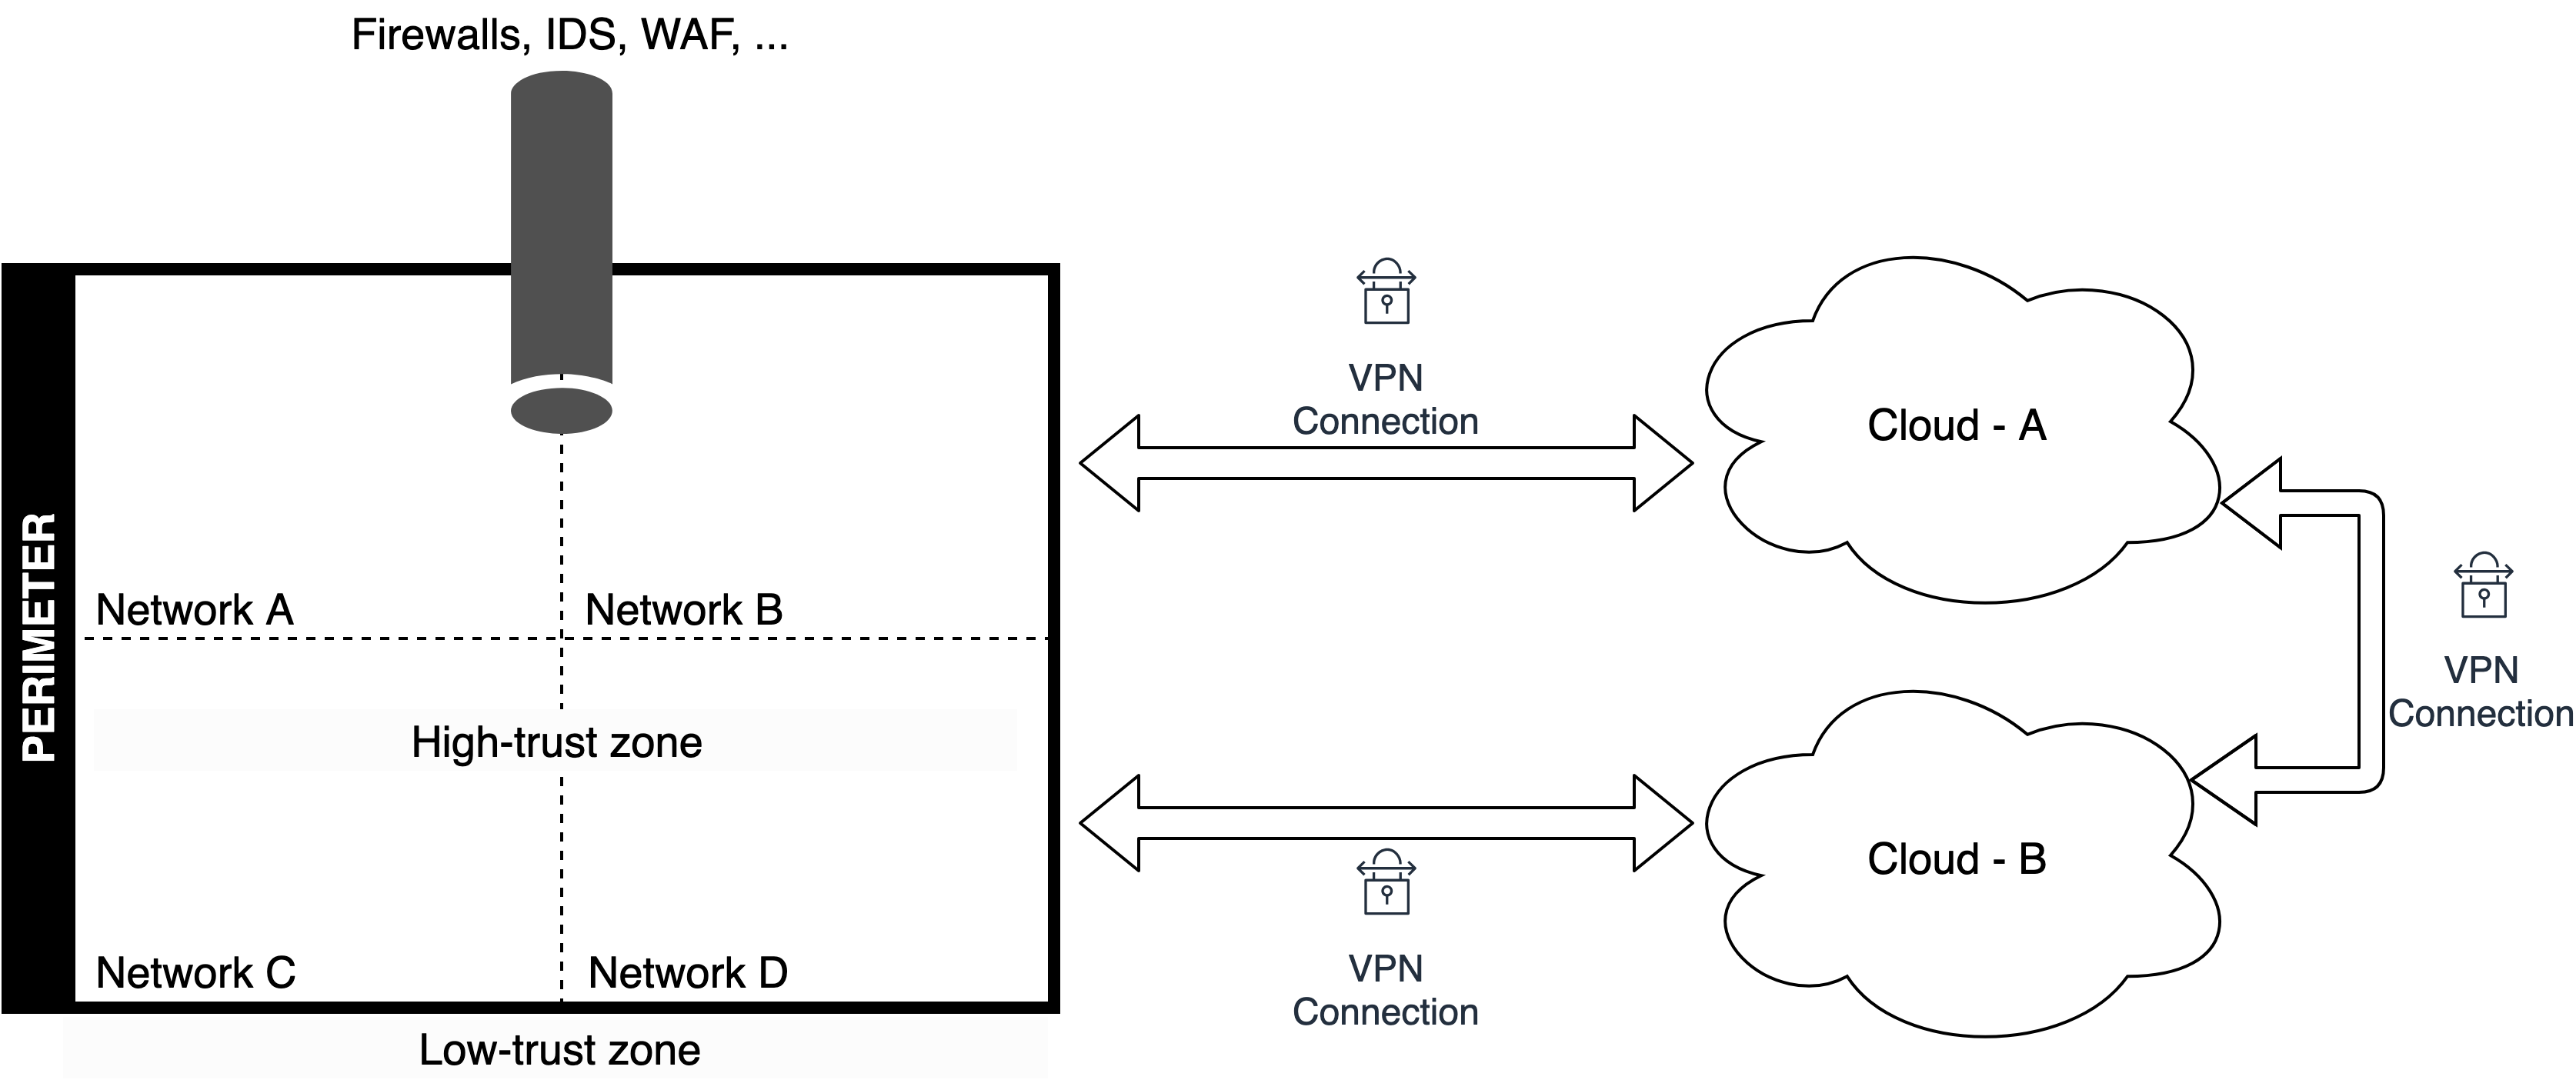
\includegraphics[width=0.9\textwidth]{images/nsip_perimeter_cloud.png}
    \caption{Combining multiple clouds with a perimeter-centric approach.}
    \label{perimeter_cloud}
\end{figure}

The acknowledgment that most of data breaches happen from the inside \cite{ref_url_verizon} brings further challenges. For example, if we look at Snowden, he was a contractor of the NSA and had VPN credentials. He had the ability to log in and access privileged systems. So this is not an attack from the outside of the organization. This is an insider threat. As we see again, it doesn't help to rely on the strength of a large perimeter, it is as in fact permeable.

Another challenge is how do we think about data protection? If we go back to the security assumption that our perimeter is keeping the attackers out, and we're assuming that everything that made it into the network is trusted. So it is all right to save unencrypted data because attackers couldn't get to it to read it. But once we change these assumptions, for example, that we don't trust all operators because they represent a potential insider threat, we care a lot more about protecting the integrity of our data. So what becomes essential is that all of the data should be encrypted.

To solve these challenges, we see that we need another low trust philosophy with little to no access to systems instead of just giving trust for being on the network. Following this low trust approach, one thing that becomes essential is secrets management, meaning how we manage (distribute, update, revoke) all of the credentials that provide access to privileged systems. For example, a running web server has the ability to connect to a database. That database has a username and password to access it. They might be hardcoded in plain text in the version control system, configuration files, or the application itself. Within the high-trust perimeter, it is all right if these credentials are easily accessible, but if we don't assume the perimeter as the ultimate line of defense, it becomes obvious that we should protect these secrets much more carefully and scope the access down. Therefore, secrets should be encrypted with access controls around them and with the possibility of auditing the access.

As we see, data breaches happen \cite{ref_url_guardian}, external attacks are relatively rare compared to internal attacks \cite{ref_url_verizon}, and consequently, it is necessary to move away from the perimeter-centric approach and to invest in prevention and mitigation. Solutions in products like Amazon AWS \cite{ref_url_aws}, Google Kubernets \cite{ref_url_gl}, and Docker \cite{ref_url_docker} have been developed within the last years to provide secrets management on an appropriate scale. In our work, we focus on the open source \textit{Vault} project \cite{ref_url_vault} which offers a vendor-independent solution, decent documentation, and is relatively popular.

\section{Secrets Management Tool}

Before we delve deeper into overall concepts of Secrets Management and give insights into how concrete Management Tools for Secrets like \textit{Vault} or the \textit{AWS Secrets Management Service} work, we define the term \textit{Secrets Management}. Furthermore, we define the term \textit{Secrets Management Tool} and separate this idea from some existing approaches.

\subsection{Definitions}

\noindent
\textbf{Secret}\newline
A \textbf{secret} is anything that grads access. More precisely, a secret is anything that can be used to authenticate or authorize. Examples for secrets are username + password, API tokens or certificates.\newline

\noindent
\textbf{Secrets Management}\newline
As described above modern applications and software systems are or will be extremely decentralized. This fact leads to three main questions that if we are able to answer to securely manage any secret information that is needed in our ecosystem: 

\begin{itemize}  
\setlength\itemsep{1mm}
\item How can a secret be distributed to its application?
\item How can a secret be updated?
\item How can a secret be revoked in case of a breach?
\end{itemize}

\noindent
Building a process around these questions and defining a lifecycle around a secret can be defined as \textbf{Secrets Management}.
\newline

\noindent
\textbf{Secrets Management Tool}\newline
A \textbf{Secrets Management Tool (SMT)} is a software tool that stores secret information in a safe way and includes all the functionality that is needed for Secrets Management. 

Tools and software solutions like \textit{Vault} or the \textit{AWS Secrets Management Service}, which will be discussed in detail in following sections, are solutions that offer functionalities for storing, distributing, updating but also for revoking and rotating secrets. Providing these key functionality these tools enable for example admin users to build a process around the three key questions of Secrets Management and so define the whole lifecycle of a secret which makes these tools SMTs.

\subsection{Non Secrets Management Tools}
When we talk about SMTs, we mean tools that fully meet the definition described above. In particular, we are not talking about solutions that fall into one of the following categories.\newline

\noindent
\textbf{Cloud Storage}\newline
Cloud storages could be used to store secrets. Storing secrets is one key feature of an SMT but since a cloud storage solutions like \textit{Dropbox} \cite{ref_url_dropbox} or \textit{ownCloud} \cite{ref_url_owncloud} doesn't include mechanisms to distribute, update or revoke secrets, a cloud storage software is no SMT in the sense of the given definition. \newline

\noindent
\textbf{Password Manager}\newline
Password managers like \textit{1Password} \cite{ref_url_1password} or \textit{KeePass} \cite{ref_url_keepass} are solutions to store and protect secret information, additionally they also provide the functionality to update a secret via a user interface. Nevertheless, these tools don't include functionality to revoke or distribute a secret which leads to the fact that these tools are no SMTs. \newline

\noindent
\textbf{Key Management Tools}\newline
Key Management Tools like the \textit{AWS Key Management Service} \cite{ref_url_aws_sms} are services that are used to manage and store encryption keys. These systems include functionality to update and distribute keys but they normally don't provide the functionality to revoke a key which is why a Key Management Tool is, in general, no SMT. In addition, these tools only manage keys which are just a subset of what we have defined as an SMT.\newline

\noindent
\textbf{Configuration Management Systems}\newline
Configuring an application almost always includes the process of setting up secrets. This is why systems like \textit{Chef} or \textit{Puppet} often include single-key encrypted storage for secrets \cite{vault_vs_chef}. Using the configuration functionality with the secret storage, these tools can be used to distribute secrets, but they don't enable us to build a real lifecycle around the key questions of secrets management. \newline

\section{Security Model}

Due to the nature of an SMT and the confidentiality of data it is managing, the security model is critical. The overall goal of the security model is to provide confidentiality, availability, integrity, accountability, authentication.

This means that stored and transmitted data must be secure from eavesdropping. Clients must be authenticated and authorized to access data or modify policies. All interactions must be traced uniquely back to the originating entity and auditable. Finally, the system must be robust against intentional attempts to bypass any of its access controls.

\subsection{Threat Model}

Applying a central SMT, we consider the following aspects as important parts of the threat model:

\begin{itemize}
\setlength\itemsep{1mm}
\item Eavesdropping on any communication. Client communication with the SMT should be secure from eavesdropping as well as communication from the SMT to its storage backend.

\item Manipulation of stored or transmitted data. Any manipulation should be detectable and cause the SMT to abort processing of the transaction.

\item Access to data without authentication or authorization. All requests must be proceeded by security policies.

\item Access to data without accountability. Before the client holds any secrets, an audit mode should enable that requests and responses must be logged.

\item Confidentiality of stored secrets. Any data that leaves the SMT to be persisted on disk must be safe from eavesdropping, meaning all stored data must be encrypted.

\item Availability of secrets in the face of failure. The SMT should support to run in a highly available configuration to avoid loss of availability.
\end{itemize}

We are not considering the following parts for the SMT threat model:

\begin{itemize}
\setlength\itemsep{1mm}
\item Protecting against memory analysis of a running SMT. An attacker that can read the memory of a running SMT instance could be able to compromise the confidentiality of the whole system.

\item Protecting against the leakage of the existence of secrets. If an attacker is able to read from the storage backend, it may be possible to observe that secrets exist, even if they are kept confidential.

\item Protecting against arbitrary control of the storage backend. If an attacker is able to run operations against the storage backend, it is possible to bypass security in any number of ways that are almost impossible to protect against. For instance, an attacker could manipulate the content of the storage backend and cause total data loss for the SMT.
\end{itemize}

\subsection{External Threats}

When we think about an SMT architecture in general, there are three distinct systems we are concerned with. The client, which is communicating to the SMT over an API, the server of the SMT which is providing an API and serving requests, and finally, the storage which is used to read and write data. 

There is no trust between the SMT and the client by default. Clients need to use, e.g. TLS, to verify the identity of the server and to establish a secure communication channel. The SMT, on the other hand, requires that a client provides a form of secret information, e.g. a token, for every request which is used to identify the client. A client that doesn't provide this information is only permitted to make login requests.

Storages should be untrusted by design. An SMT should encrypt all data leaving it using, e.g. a 256-bit Advanced Encryption Standard (AES). When data is read, the SMT should verify during the decryption process if any manipulation took place.

\subsection{Internal Threats}
\label{sec:internal_threats}

The critical security concern is that attackers gain access to secrets they are not authorized to. This is an internal threat if the attacker already has a certain level of access to the SMT and is able to authenticate. According to this thread, the following methods could be used to reduce that risk.

A certain authentication method, which is used to verify the identity of the client, has to be chosen when a client authenticates for the first time. This method has to be configured by operators of the SMT ahead of time and could be a list of associated ACL policies. The SMT could then randomly generate a token, map it to the policy list, and return it to the client. On each request, a client provides this token. The SMT then validates the token, checks if it is revoked or expired, and generates an ACL based on the associated policies. Thereby, a strict deny or whitelist enforcement can be used, meaning unless an associated policy allows for a given action, it will be denied.

By using a secret sharing technique, like Shamir's Secret Sharing which we describe in \autoref{sec:shamir}, we avoid the need to place absolute trust in the holder of the master key and avoid storing the master key at all. The master key is only retrievable by reconstructing the shares and these are not useful for making any requests.

\section{Encrypting Secret Information}
\label{sec:external_threats}

An SMT obviously has to store secret information, e.g. credentials and access tokens. As described in \autoref{sec:external_threats}, this information has to be protected in some way, for example by using a well-known standard for encryption like the AES.

Using AES or any other encryption scheme leads to the fact that an encryption key (EK) is generated which directly leads to questions: How do we manage the EK? Who should hold the EK? Who should have access to the EK?

These are central questions in SM that are not easy to answer since the EK protects all secret information and is consequently the most sensitive information of an SMT.

As a first approach, we could argue: The higher the number of key holders the higher the possibilities of a key misuse and also the higher the possibility that unauthorized users get access to the key. Therefore, a possible consideration could be to only give the encryption key to a single person who is then the most important and trusted party, e.g. the CEO or the owner of a company. 

This solution is simple but has some weak points:
For example, the system is not protected against the situation where the holder of the key turns rogue. Since there is only one party having full power over all secret information it is easy for this party to cause great harm, e.g. manipulate or delete secret information.
Another problem of having this single point of failure is if the access to the encryption key gets lost. Possible scenarios are that the holder of the key passes away, the key is stolen physically, e.g. the storage medium is stolen or the key holder's system gets hacked.

After discussing these weak points, we come to the conclusion that giving the key to a single user is not an option for an SMT. Thus, we should try to split the secret into multiple pieces and distribute the risk.

\subsection{Shamir's Secret Sharing}
\label{sec:shamir}

To reduce the impact of a rogue key holder, it is convenient to split the key in some way. Redundancy is another vantage point to prevent the situation of a stolen or lost key. Overall, we want to avoid the need to place absolute trust in the holder of the EK as already mentioned in \autoref{sec:internal_threats}.

One solution we can use to address these points is proposed by Adi Shamir in his article ``How to Share a Secret'' \cite{shamir}. He describes the definition and a simple solution for a so called $(k,n)$ \textit{threshold scheme} which can be used to split a secret into multiple shares and at the same time generate redundant information.
\newline

\noindent
\textbf{Definition of a $(k,n)$ \textit{threshold scheme}} according to Shamir:
\newline

\noindent
The overall goal of a $(k,n)$ \textit{threshold scheme} is to divide some Data $D$ into $n$ pieces $D_1,...,D_n$ in such a way that
\begin{itemize}
\setlength\itemsep{1mm}
\item[] (1) The knowledge of any $k$ or more $D_i$ pieces makes $D$ easily computable and
\item[] (2) the knowledge of any $k-1$ or fewer $D_i$ pieces leaves $D$ completely undetermined.
\end{itemize}

\noindent
\textbf{Main Idea of Shamir's simple $(k,n)$ \textit{threshold scheme}}:
\newline

\noindent
Given $k$ points $\{(x_1,y_1),...,(x_k,y_k)\}$ in a two dimensional plane there is one and only one polynomial $q(x)$ of degree $k-1$ such that $q(x_i) = y_i$ for all $k$ points.
\newline

\noindent
\textbf{How Shamir's Secret Sharing can be used to split the encryption key of SMT}:
\newline

\noindent

\begin{enumerate}
    \setlength\itemsep{1mm}
    \item An AES EK is generated that is used to encrypt all secret information managed by the SMT.
    \item A second key, the so called master key (MK), is generated and used to encrypt the AES EK.
    \item Values for $\bm{k}$ and $\bm{n}$ are chosen. In this context they have the following meaning: 
\begin{itemize}
    \item $\bm{k}$ - the number of shares that should be necessary to access the key
    \item $\bm{n}$ - the overall number of shares
\end{itemize}
    \item The MK is encoded as a number which leads to the value $\bm{a_0 = enc(MK)}$.
    \item $\bm{k-1}$ random integers ($\bm{a_1,...,a_{k-1}}$) are selected to create in combination with the encoded MK ($\bm{a_0}$) a polynomial of degree $\bm{k-1}$:\newline
     $\bm{q(x) = a_0 + a_1x + a_2x^2 + ... + a_{k-1}x^{k-1}}$.
    \item $\bm{n}$ points form $\bm{q(x)}$: $\bm{D_1 = q(1), ..., D_n = q(n)}$ are calculated and used as the key shares which are given to different users.
\end{enumerate}

To reconstruct the MK which is used to decrypt the EK, at least $\bm{k}$ key shares $\bm{D_i}$ are required. The polynomial $\bm{q(x)}$ can be reconstructed via interpolation which gives us the encoded \textbf{MK} $\bm{enc(MK) = a_0 = q(0)}$. A visualization of that scenario with $\bm{n = 5}$ can be seen in \autoref{shamir}.
\newline

\noindent
\textbf{Important note}:
\newline

\noindent
Using the method described above with \textit{normal} integer arithmetic, leads to the problem that an attacker gains a lot of information with every additional key share he has access to. In consequence \textit{normal} integer arithmetic should \textbf{not} be used for applying this secret sharing scheme. Instead finite field/modulo arithmetic can be used as proposed by Shamir \cite{shamir}.

\begin{figure}
    \centering
    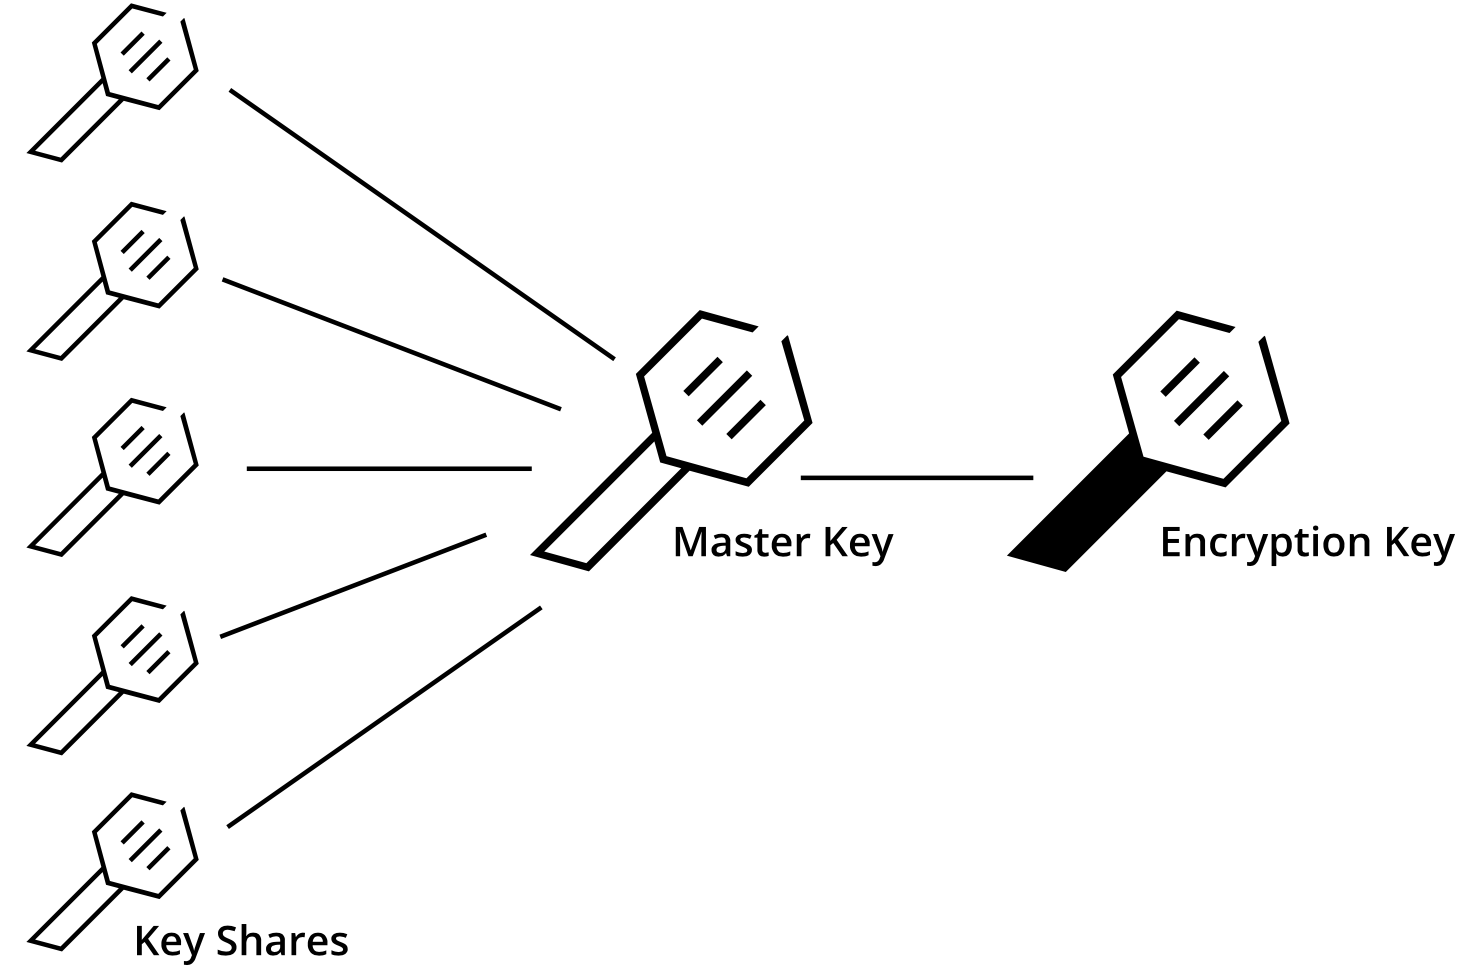
\includegraphics[width=0.8\textwidth]{images/shamir.png}
    \caption{Using Shamir's Secret Sharing to secure an encryption key.}
    \label{shamir}
\end{figure}

\subsection{Scenarios and how to solve them using Secret Sharing}

To show how Shamir's Secret Sharing can be applied, we present some use cases which discuss some desired scenarios.
\newline

\begin{itemize}
    \setlength\itemsep{1mm}
    \item \textbf{Case 1: Users with equal power} \newline
    
    \textbf{Goal:} We want to have $u$ users with equal power, $x$ of this users together should have the power to reconstruct the secret. \newline
    \textbf{Implementation:} Use a $(k,n)$ \textit{threshold scheme} as presented above with $k = x$ and $n = u$ and give every user a single share of the secret.\newline
    \textbf{Protection level:} The system is safe as long as less than $k = x$ users are malicious.
    \newline
    
    \item \textbf{Case 2: One user with more power than all other users} \newline
    
    \textbf{Goal:} We want to have one user that has more power than all other users, the others should have an equal amount of power. More formal: We have $u$ users, one user should only have to ask $y$ other users to get access to the full secret. All other users should have to ask at least $z>y$ other users. \newline
    \textbf{Implementation:} Use a $(k,n)$ \textit{threshold scheme} presented above with $k = z+1$ and $n = u + k - y - 1 = u + z - y$.
    
    This selection gives us one key share for every \textit{normal} and $k - y$ key shares for the user with more power. Since $k = z+1$, a \textit{normal} user has to ask at least $z$ other users for reconstruction of the secret but the one user with more power holds $k - y$ key shares and has to ask only $y$ other users. \newline
    \textbf{Protection level:} The system is safe as long as less than $y+1$ users are malicious.\newline
    
    \item \textbf{Case 3: One user with independent access to the secret} \newline
     
     \textbf{Goal:} We want to have a user that is able to reconstruct the secret without the help of other users. All other users should have equal power. More formal: We have $u$ users, one user should have to ask $0$ other users to get access to the full secret. All other users should have to ask at least $z>0$ other users. \newline
     \textbf{Implementation}: We apply the implementation from case 2 with $y = 0$ which gives us $k = z+1$ and $n = u + k - 1 = u + z$. We give k of the $n$ shares to the one user that should have independent access to the key which leaves us with one key share for every other user. Consequently, the user having $k$ key shares don't has to ask any other user to reconstruct the MK. All other users have one key share and have to ask $z$ other users.  \newline
     \textbf{Protection level:} The system is safe as long as the one powerful user is not malicious and as long as less than $k$ of the other users are not malicious.\newline
     
     \item \textbf{Case 4: Multiple users with different power:} \newline
     
     If we want to have multiple different users with multiple different levels of power, we simply create as many keys as we need and hand out a number of key shares to the users that correlates to their level of power. In this case it is important to carefully think about who can access the secret in which scenarios.
\end{itemize}

\noindent
\textbf{The importance of the value of the parameter $\bm{u}$ in case of unequally distributed power}:
\newline

In case 2 and 3, we give a single user more power than others. In these cases (also in case 4), we have to be especially careful how we choose the value of the parameter $u$ because if we don't, it might come to the situation where it is not possible to reconstruct the secret without asking the single user with an increased level of power which would make the whole process of secret sharing useless. To avoid this scenario, we have to ensure that the value for $u$ is greater than the value for $k$.
\newline

\noindent
\textbf{Maintain and manage secret shares}:
\newline

\noindent
Imagine the Secret Sharing Scheme is used to distribute secret shares over employees of a company. It is likely that we have to \textbf{create a new key share}: a new employee joins the company, a key share gets public and has to be \textbf{revoked/renewed}, or secrets should be regularly \textbf{rotated} because of security concerns. In the following, it is described how to handle these scenarios.

\begin{itemize}
    \setlength\itemsep{1mm}
    \item \textbf{Create an additional key share} \newline
    To create a new additional key share, we collect $k$ or more of the existing key shares to reconstruct our polynomial $q(x)$. We can now select as many new tuples $(x_i,q(x_i))$ as we need and give them as key shares to the new user(s). 
    
    Note that we don't need to change our secret/MK and in addition, all key shares that existed before are still valid. 

    \item \textbf{Revoke/Renew a single key share} \newline
    First of all we denote the tuple we want to invalidate with $(x_{inv},q(x_{inv}))$.
    To revoke that tuple, we select a new polynomial $q'(x)$ so that $q(0) = q'(0)$ and $q(x) = q'(x)$ for all values $x$ that are part of a tuple that should stay valid. At the same time we make sure that $q(x_{inv}) \neq q'({x_{inv}})$. Now we select a new tuple $(x_{new},q'(x_{new}))$ and replace $(x_{inv},q(x_{inv}))$ by this tuple.
    
    Note that we also don't need to change our secret/MK ($q(0) = q'(0)$) and that all key shares that existed before are still valid. 
    
    \item \textbf{Rotate the Secret/Master Key} \newline
    If we want to rotate the hole secret, we select a completely new polynomial $q'(x)$ so that $q(x) \neq q'(x)$ for all $x$ that are currently used in tuples as well as for $x = 0$ (the secret itself). 
    
\end{itemize}

\section{Deliver secrets}

Above we discussed how to encrypt the EK of a secrets management software solution. In the following, we will discuss the challenge how does an user/application authenticate itself against an SMT for the first time?

Thinking of a human user (Alice) who should authenticate against an SMT to get an access token, this is no problem at all: We provide Alice with some secret information (e.g. username and password) via a secure channel (e.g. a company internal letter). Having this information, Alice is able to present it to the SMT and authenticate against it.

\subsection{The Secret Zero Problem}

Thinking of an application that should authenticate against an SMT for the first time is not that easy to solve. Since we don't want to use hardcoded credentials in the sourcecode or environment variables, the application has at the very beginning no information that it can present to the SMT to prove its identity. This problem, that the SMT has to establish trust to another application for the first time is known as the \textit{Secret Zero Problem}, \textit{Bootstrapping Problem} or \textit{Last Mile Problem}.

In general, there is no solution for this problem because an application has no other way than providing information to prove its identity but somehow the application has to get this information which leads to a chicken or egg problem.
Nevertheless, techniques exist to deliver an initial secret to an application and at the same time minimize the risk of attacks where, for example, a malicious user gets access to this initial information. We want to present one technique in an abstract way and discuss the concept of \textit{Response Wrapping}. How this idea is implemented and used in \textit{Vault} is described later in \autoref{sec:sec_intro}. \newline

\noindent
\textbf{Deliver Secret Zero} \newline
\noindent

\noindent
Lets assume the following setting:

\noindent
A new machine is booted running an application \textbf{\textit{A}}.
It needs some credentials to communicate with other services that it gets form an SMT \textbf{\textit{S}}. Now \textbf{\textit{A}} has to get an authentication token \textbf{\textit{T}} from \textbf{\textit{S}}.

\begin{enumerate}
    \setlength\itemsep{1mm}
    \item \textbf{\textit{S}} receives the request to create an authentication token \textbf{\textit{T}} for \textbf{\textit{A}}
    \item \textbf{\textit{T}} (which is the actual response for \textbf{\textit{A}} to the request) is serialized
    \item A new single use token (\textbf{\textit{SUT}}) is created
    \item The serialized version of \textbf{\textit{T}} is stored at a dedicated location in memory that only can be accessed by using the \textbf{\textit{SUT}}.
    \item The \textbf{\textit{SUT}} is injected (for example via a trusted deployment service) into \textbf{\textit{A}}
    \item \textbf{\textit{A}} sends the \textbf{\textit{SUT}} to \textbf{\textit{S}}
    \item \textbf{\textit{S}} looks up the serialized version of \textbf{\textit{T}} by using the \textbf{\textit{SUT}} and sends it back to \textbf{\textit{A}}
\end{enumerate}

\noindent
The idea of not sending the response to a request directly to the other party but instead sending a token which can be used to get the real response later is called \textbf{\textit{Response Wrapping}}. Thereby, we wrap the response by creating a token and store the response in a dedicated place in memory that only can be accessed by presenting this token.

Why this is a better way than injecting the token directly to the application is also discussed in \autoref{sec:sec_intro}.

\section{Vault Architecture}

In the following \autoref{vault_architecture}, we give a brief overview of the underlying \textit{Vault} architecture. For further reading and insides, we recommend the detailed documentation \cite{ref_url_vault_architecture}.

\begin{itemize}

\setlength\itemsep{1mm}

\item \textbf{Core} - The \textit{Vault} architecture exhibits a central core which has many responsibilities, including the lifecycle management ensuring requests are processed correctly. Additionally, there are many extension points offered that can be used to adjust the system to its environment.

\item \textbf{Authentication backend} - It provides clients the possibility of authenticating from different systems. As an example, the AWS authentication plugin can be used to authenticate an EC2VM when it's booting. But other authentication options like LDAP or Active Directory can also be applied.

\item \textbf{Auditing backends} - The auditing backends provide the possibility of streaming requests and responses out and give a trail of who's done what. This stream can then be consumed by any other audit software, e.g. Splunk or Syslog.

\item \textbf{Storage backends} - The storage backends are responsible for storing encrypted data which can be quite variable. It could be a standard RDBMS, a KV store, or a cloud-managed database. The goal is to provide highly available durable storage systems so that the loss of one of these can be tolerated.

\item \textbf{Barrier} - All traffic that is sent between \textit{Vault} and the storage backend has to pass the barrier. It ensures that only encrypted data is persisted, and verifies the decryption.

\item \textbf{Secret engines} - The secret engines provide access to different secrets which come in different forms. For example, a key-value store that stores static credentials like username and password. A more sophisticated method is to create secrets dynamically on demand. That is where different plugins can be used. These engines dynamically manage credentials for different systems, e.g. for MySQL, Postgres, Oracle, RabbitMQ, SSH.

\item \textbf{Server} - The server is a long-running single-instance exposing a restful JSON API which the client can use for interaction and making it relatively easy to integrate with other applications. To increase availability, the \textit{Vault} instance can be replicated and one instance will be elected as the leader. All client requests are then sent to the leader. Even when a client sends requests to a non-leader, they will be transparently forwarded to the active leader. If a node dies, it will be detected and a new leader will automatically be elected.

\end{itemize}

\begin{figure}
    \centering
    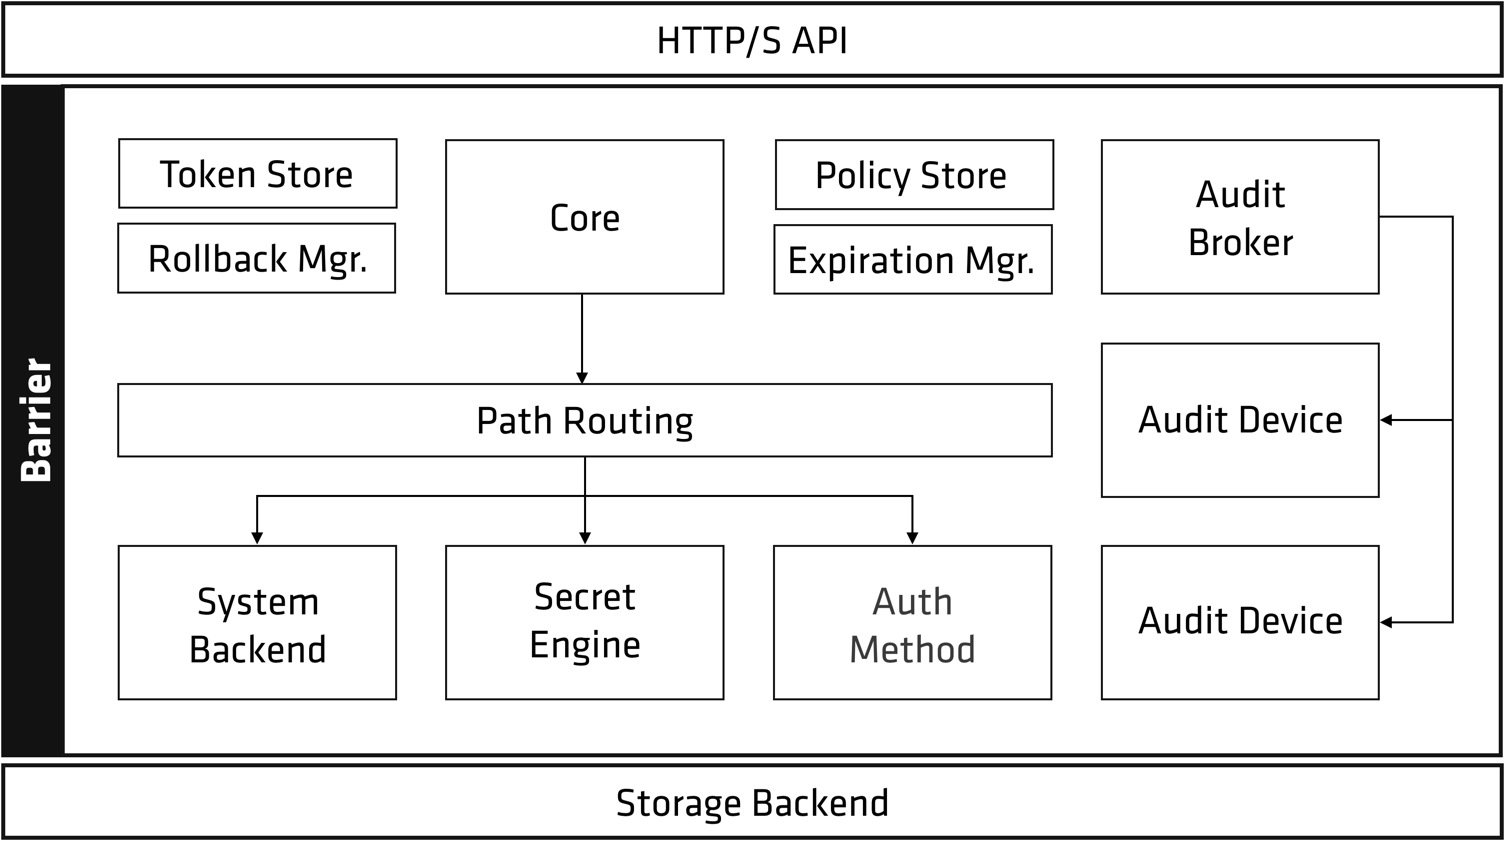
\includegraphics[width=0.8\textwidth]{images/vault_architecture.png}
    \caption{An overview of the \textit{Vault} architecture}
    \label{vault_architecture}
\end{figure}

\newpage

\subsection{A brief link to AWS}
Above we gave an overview over the architecture of the secrets management software \textit{Vault}. Since information provided us with insights into \textit{AWS Key Management Service} (AWS-KMS) \cite{aws-kms} as well as how this service is used by the \textit{AWS Secrets Management Service} (AWS-SMS) \cite{aws-sms}, we want to present how AWS-KMS, AMS-SMS and the \textit{AWS Identity and Access Management} (AWS-IAM) work together to implement a service that is similar to \textit{Vault}. Especially, we want to analyze where key components presented in the \textit{Vault} architecture can be found in the AWS setup.

An overall visualization of how AWS-KMS, AWS-SMS, and AWS-IAM refer to each other is given in \autoref{aws_architecture}. 

\begin{figure}
    \centering
    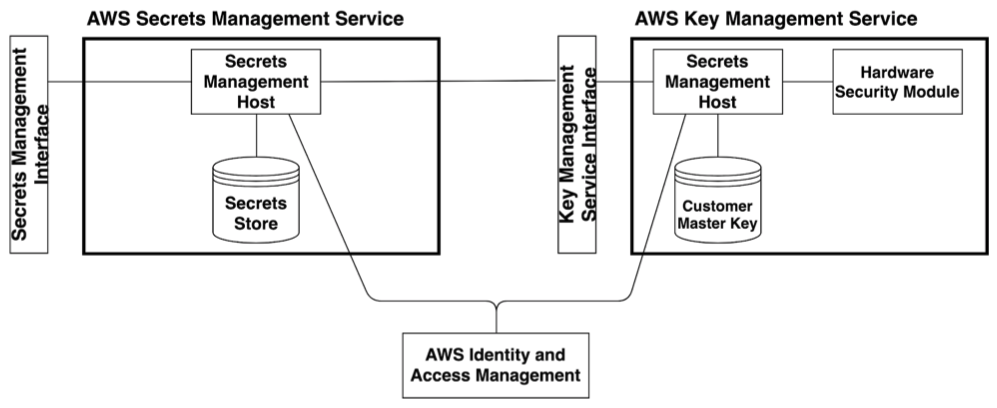
\includegraphics[width=\textwidth]{images/aws.png}
    \caption{The AWS Secrets Management Service using the AWS Key Management Service and the AWS Identity and Access Management Service.}
    \label{aws_architecture}
\end{figure}

\begin{itemize}
    \setlength\itemsep{1mm}
    \item \textbf{AWS Secrets Management Service (AWS-SMS)}\newline
    The AWS-SMS provides all the secrets management related functionality for the users. It handles the request flow and is responsible for encryption and storing secret information using the AWS-KMS and AWS-IAM. In \autoref{aws_architecture}, it consists of the user interface, a host component which includes all the logic and an secrets store for saving the encrypted secrets.
    \item \textbf{AWS Key Management Service (AWS-KMS)}\newline
    The AWS-KMS is responsible for managing encryption keys for the secrets, also called data keys. These keys are protected by another key, the customer master key. As the AWS-SMS, this service consists of a host handling the request flow and a component which is responsible for storage. In addition, AWS-KMS also includes a FIPS 140-2 \cite{fips140} proven multichip standalone hardware component which is just there to process cryptographic operations. 
    \item \textbf{AWS Identity and Access Management (AWS-IAM)}\newline
    The AWS-IAM is used by both services to manage access rights and check user permissions.
\end{itemize}

\noindent
\textbf{Encrypt and store a secret Value}:
\begin{enumerate}
    \setlength\itemsep{1mm}
    \item AWS-SMS gets the request to store a secret value.
    \item AWS-SMS requests a 256-bit AES key from the AWS-KMS.
    \item AWS-KMS returns a 256-bit AES key in plain-text as well as an encrypted version of the key that can only be decrypted by AWS-KMS.
    \item AWS-SMS uses the AES algorithm together with the received key to encrypt the secret.
    \item AMS-SMS deletes the plaintextversion of the AES key.
    \item AWS-SMS stores the encrypted secret, the encrypted version of the AWS key and related metadata.
\end{enumerate}

\noindent
\textbf{Decrypt a secret Value}:
\begin{enumerate}
    \setlength\itemsep{1mm}
    \item AWS-SMS gets the request to return a secret value.
    \item AWS-SMS passes the encrypted version of the related AES key to AWS-KMS.
    \item AWS-KMS decrypts the AES key and gives the plaintext version of it back to AWS-SMS.
    \item AWS-SMS uses the AES algorithm in combination with the key to decrypt the secret value.
\end{enumerate}

\subsection{Comparison to Vault Architecture}

\autoref{aws_architecture_mapping} shows a rough mapping of the AWS Services and their functionalities to a reduced version of the \textit{Vault} architecture.

In \textit{Vault}, the Core offering an API is responsible to handle the request flow. Leaving out the encryption and authentication part of that task the core accesses the secrets engine and the Storage Backend. Mapping this functionality to the AWS architecture, we will have pretty much the same functionality and components as the AWS-SMS (see red selection).

Everything related to the authentication of users is managed by the Token- and Policy Store in combination with different Auth Methods and an optional Authentication Backend. In the AWS setup, these tasks are fulfilled by the AWS-IAM (see green selection).

The only \textit{Vault} component that we can not map to an AWS service is the Barrier. Since it is responsible for everything related to encryption the most fitting component would be the AWS-KMS (see blue selection). The difference between these two is that the Barrier in \textit{Vault} is more of an abstract concept which protects the \textit{Vault} system itself but the AWS-KMS is a service which can be used as a standalone service having an hardware module for encryption.

\begin{figure}
    \centering
    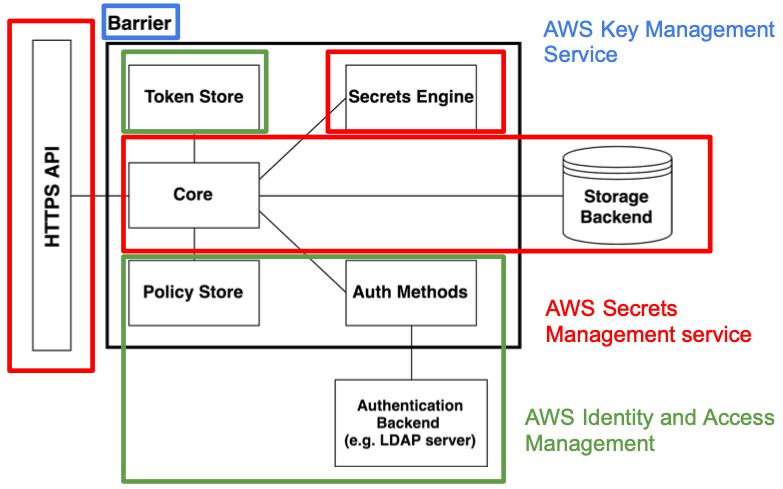
\includegraphics[width=0.8\textwidth]{images/aws_mapping.png}
    \caption{Mapping of AWS components to \textit{Vault} architecture}
    \label{aws_architecture_mapping}
\end{figure}

\newpage

\section{Practical Experience}
To understand \textit{Vault} and its concepts better, we had some hands-on experience and recorded it. To make it more comprehensible, we put our setup and all dependencies into docker containers. In the following, we give some examples which can be easily reconstructed following along the instructions of the repository \cite{ref_url_repository}.

\subsection{Initializing and unsealing a Vault server}
If we start \textit{Vault} for the first time and want to see its status, we execute: 

\begin{lstlisting}[language=bash]
$ vault status
Key                Value
---                -----
Seal Type          shamir
Initialized        false
Sealed             true
Total Shares       0
Threshold          0
Unseal Progress    0/0
Unseal Nonce       n/a
Version            n/a
HA Enabled         false
\end{lstlisting}

We see that we are connected to the \textit{Vault} server, but it is not yet initialized. The next step is to initialize the server: 

\begin{lstlisting}[language=bash]
$ vault operator init
Unseal Key 1: Mxv+QTYZeZnc+EtZIbcILzNkJp/Nm6T2HqBhtsCIis7u
Unseal Key 2: OY+88n9kruoxP2u7ieHzS12K6NE9tIqxnKqd6YjxNCeV
Unseal Key 3: jjjRGuGB09frPT9s4aW3ov3mIxy1F4o+GiX052dkHhxW
Unseal Key 4: OoeVb1zjgKRZfy3kDZme7GJe0F0cdW/QbBDTKiq59XcX
Unseal Key 5: +xiOtgsnVUaw2L3NasGjHvaFVY/7C8mZM+5c4KYoDKAE

Initial Root Token: s.iQ8fqNzZRZiZGX0P0qZjqAyw
...
\end{lstlisting}

This is a critical step that displays the unseal keys. Therefore, Sharmir's Secrets Sharing is applied which we describe in \autoref{sec:shamir}. Each unseal key is a shard of the master key. It is very important that these unseal keys be stored in a secure separate locations from each other.  Now let's try to log in with the root token:

\begin{lstlisting}[language=bash]
$ vault login s.iQ8fqNzZRZiZGX0P0qZjqAyw
Error authenticating: error looking up token

URL: GET http://vaultserver:8200/v1/auth/token/lookup-self
Code: 503. Errors:

* error performing token check: Vault is sealed
\end{lstlisting}

We get an error, because \textit{Vault} is currently sealed. Our next step is to unseal \textit{Vault}. In order to do that we use the command: 

\begin{lstlisting}[language=bash]
$ vault operator unseal
Unseal Key (will be hidden):
\end{lstlisting}

\textit{Vault} is needing three of the unseal keys to be unsealed. After we entered three keys, we see that sealed is false and \textit{Vault} is unsealed:

\begin{lstlisting}[language=bash]
$ vault operator unseal
Unseal Key (will be hidden):
Key             Value
---             -----
Seal Type       shamir
Initialized     true
Sealed          false
Total Shares    5
Threshold       3
Version         1.1.0
Cluster Name    vault-cluster-9c9491b2
Cluster ID      cce2ce83-8d3e-a9c9-a342-27598fd666df
HA Enabled      false
\end{lstlisting}

Now we are able to login using the root token.

\subsection{Dynamic Credentials}

In order to create dynamic credentials on demand, we need to setup the Database Secrets Engine first.

\subsubsection{Database secrets engine -} Perhaps contrary to their name, database secrets engines don't actually store secrets in a database, though that may seem like their natural function. In fact, they act as an authentication mechanism to supported databases. Most databases support username/password authentication. The password is a secret that must be generated then protected. Database username/password combinations are often stored in build configurations, continuous integration systems, or configuration management systems. 

The \textit{Vault} Database Secrets Engine provides a replacement for all these methods by integrating directly with supported databases, as shown in \autoref{practical_dynamic_secrets}. \textit{Vault} becomes an alternative authentication mechanism for the database: 

\begin{figure}
    \centering
    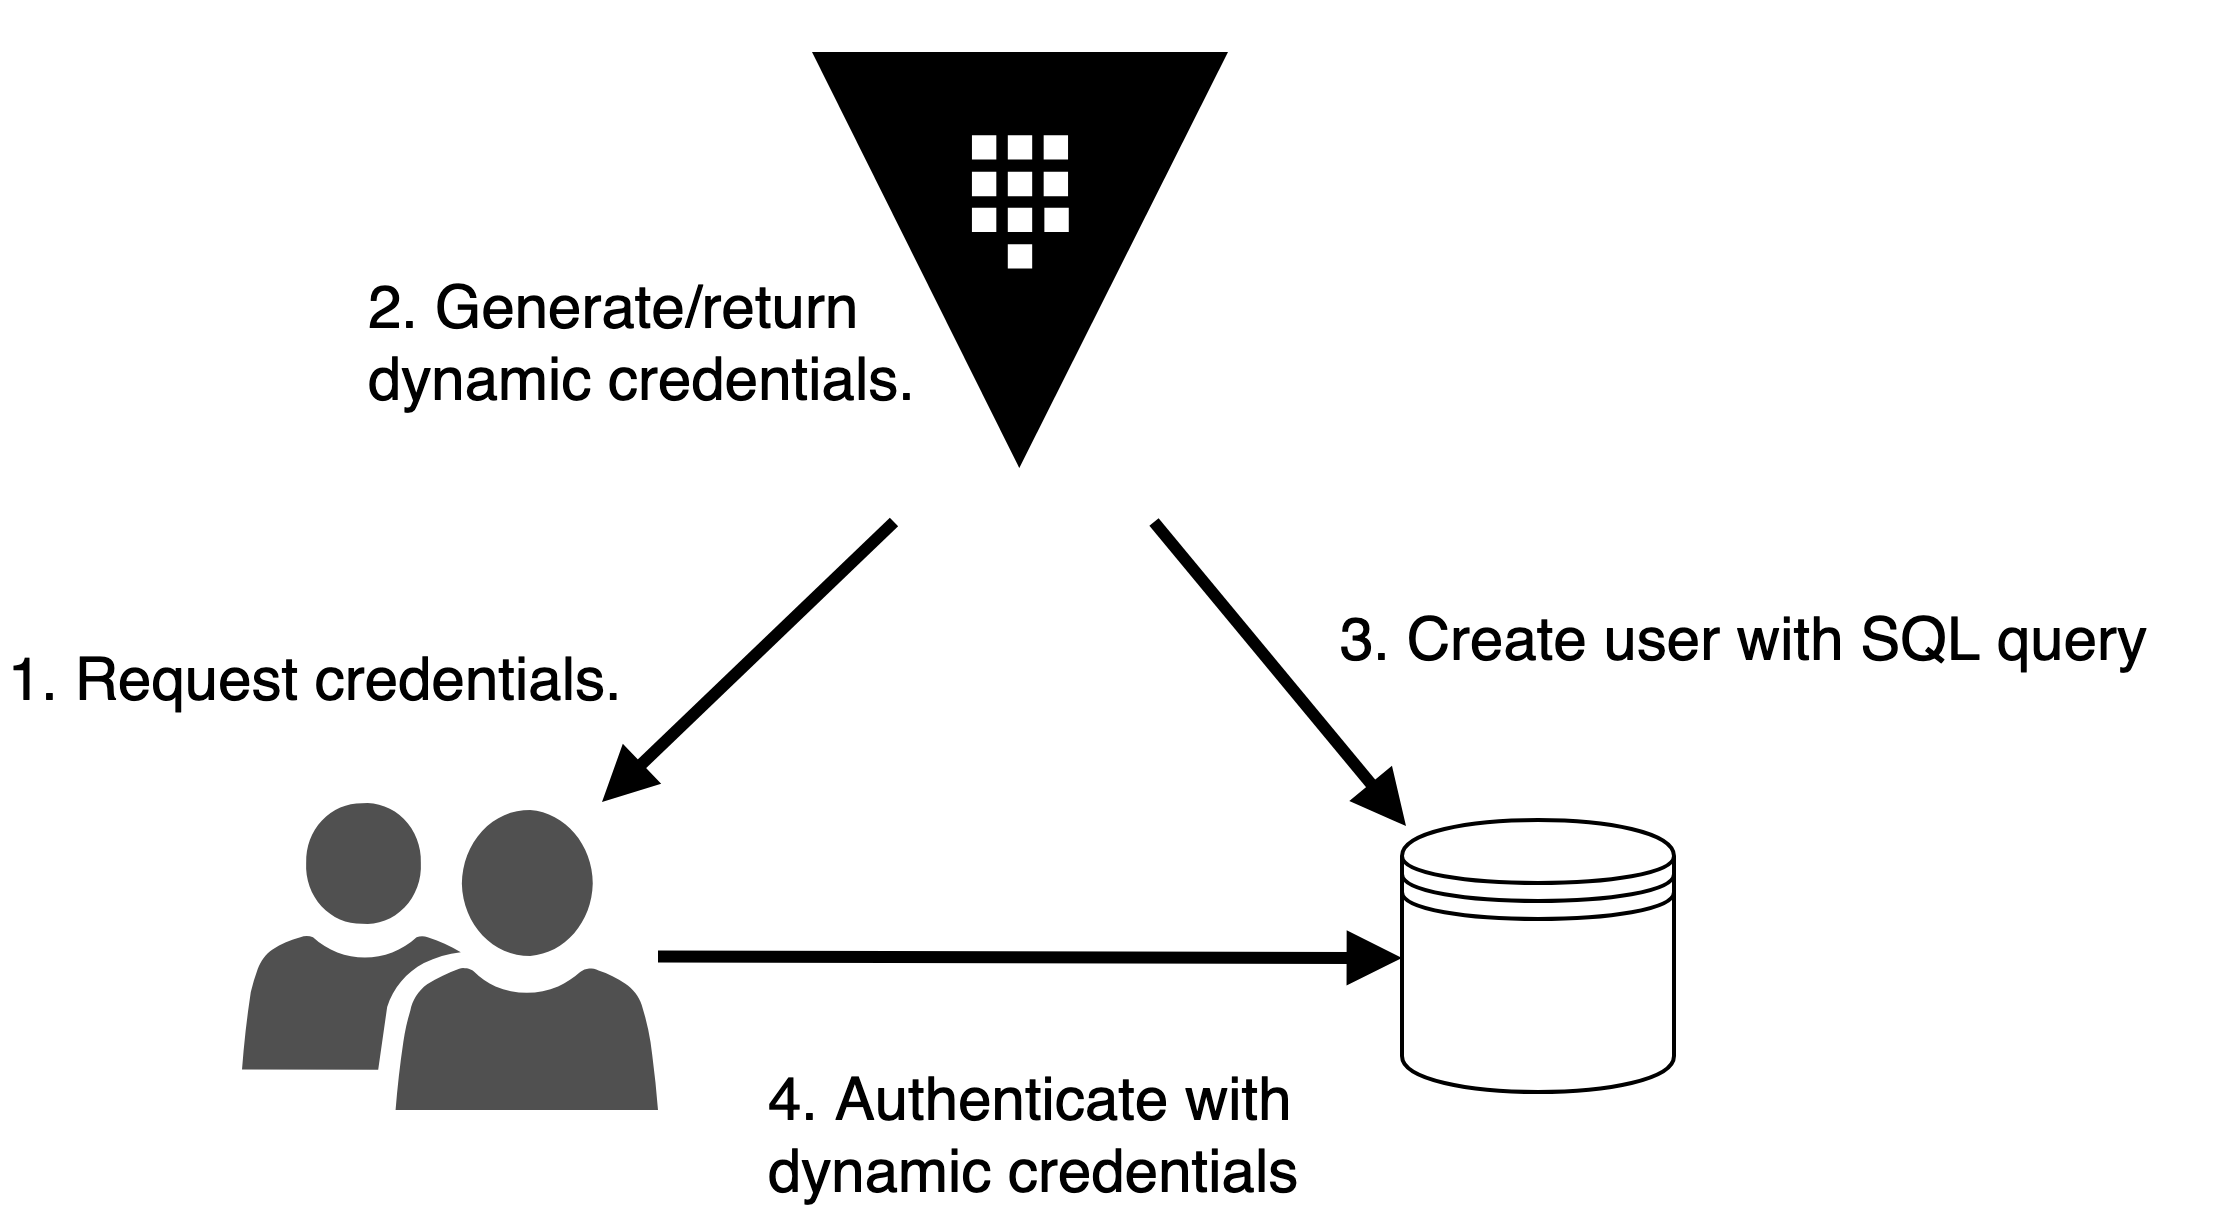
\includegraphics[width=0.8\textwidth]{images/nsip_practical_db_secret_engine.png}
    \caption{Dynamic credentials on demand for a SQL db.}
    \label{practical_dynamic_secrets}
\end{figure}

\begin{enumerate}
    \setlength\itemsep{1mm}
    \item Database clients authenticate to \textit{Vault}, then request database credentials.
    \item \textit{Vault} generates the credentials as a dynamic secret. The secret doesn't exist until it's read.
    \item \textit{Vault} then executes a query on the database  creating a user with the username/password secret combination it generated.
    \item The username and password are returned to the \textit{Vault} client and the client can then use the username and password to authenticate to the database.
\end{enumerate}

When the secret lease is up, \textit{Vault} connects to the database and removes the user it created, thus revoking the credentials to the database. In the following, we setup \textit{Vault} to serve as an authentication mechanism to a \textit{MariaDB} database.

\subsubsection{Configuring the database secrets engine -} Our first step is to enable the database secrets engine: 

\begin{lstlisting}[language=bash]
$ vault secrets enable database
Success! Enabled the database secrets engine at: database/
\end{lstlisting}

The next set of commands are rather lengthy, so we saved them in \textit{setup\_\allowbreak commands.txt} under the \textit{mariadb} folder. The first command, writes a configuration to the database secrets engine. The path is \textit{database/config/nsip-mariadb}, which is the name we have given to this configuration. The plug-in name is \textit{mysql-database-plugin}, which is compatible with \textit{mariadb}. The connection URL, is a templated connection string that is used by \textit{Vault} to connect to the database. The username and password are injected when \textit{Vault} calls out to the database. \textit{Mariadb:3306} is the URL. The \textit{allowed\_roles} are \textit{datareader} and \textit{datawriter}, which we will be using to connect to the database. These are the roles that are allowed to create credentials using this configuration, and the username and password, \textit{root} and \textit{mysql}, are the username and password to the mysql database used to make the connection. 

The next two commands create roles in the database secrets engine. The path here is \textit{database/roles/datareader}, which is the name of the role. The db name \textit{nsip-mariadb}, matches the configuration we created earlier. The creation statement, is this statement that is used to create the user in the database when credentials are generated, \textit{CREATE USER '\{\{name\}\}', IDENTIFIED BY '\{\{password\}\}, GRANT SELECT}. Grant select is a SQL command that grants read only access to a database. The \textit{datawriter} is similar, except in this case it grants all, which is create, read, update, and delete. The next two parameters are the default time to live, and the max time to live. These tokens have a default time to live of one hour, which can be renewed up to 24 hours.

\subsubsection{Policies and credentials with the database secrets engine -} Our next step is to upload policies for the \textit{datareader} and \textit{datawriter}. They are essentially the same, they both grant access to the path in the database secrets engine that generates the credentials:

\begin{lstlisting}[language=bash]
path "database/creds/datareader" {
    policy = "read"
}

path "database/creds/datawriter" {
    policy = "read"
}
\end{lstlisting}

We can upload them and create credentials with the following commands:

\begin{lstlisting}[language=bash]
$ vault policy write datareader datareader.hcl
Success! Uploaded policy: datareader

$ vault policy write datawriter datawriter.hcl
Success! Uploaded policy: datawriter

# Create a token for this role
$ vault token create -policy=datareader
Key                  Value
---                  -----
token                s.dZO7MF7oGlThDOfHLwP7wxuE
token_accessor       1Vv62YCBFnit20ciUMgRPSbO
token_duration       768h
token_renewable      true
token_policies       ["datareader" "default"]
identity_policies    []
policies             ["datareader" "default"]

# Login in as the datareader and generate credentials
$ vault read database/creds/datareader
Key                Value
---                -----
lease_id           database/creds/datareader/WWblpx3...
lease_duration     1h
lease_renewable    true
password           A1a-4zmkaOvK6PTD9izI
username           v-token-datareader-NrUg6RnIZX46o
\end{lstlisting}

\textit{Vault} has generated a username and password that we can use to login to the database using the \textit{MySQL CLI} to connect to the \textit{MariaDB} database. If we try to create a database, the access is denied. The \textit{datareader} doesn' t have permissions to write data. But if we repeat these steps with the \textit{datawriter}, we are able to manipulate data. 

\subsection{Secure Introduction}
\label{sec:sec_intro}

Let's assume that we want to deploy an application with a static username and password. We might, for example, be connecting to a database that is not supported by the database secrets engine. How do we securely automate the process of delivering secrets to an application on deployment? 

\subsubsection{Approaches -}In \autoref{practical_sec_intro_1}, we propose a solution: 

\begin{figure}
    \centering
    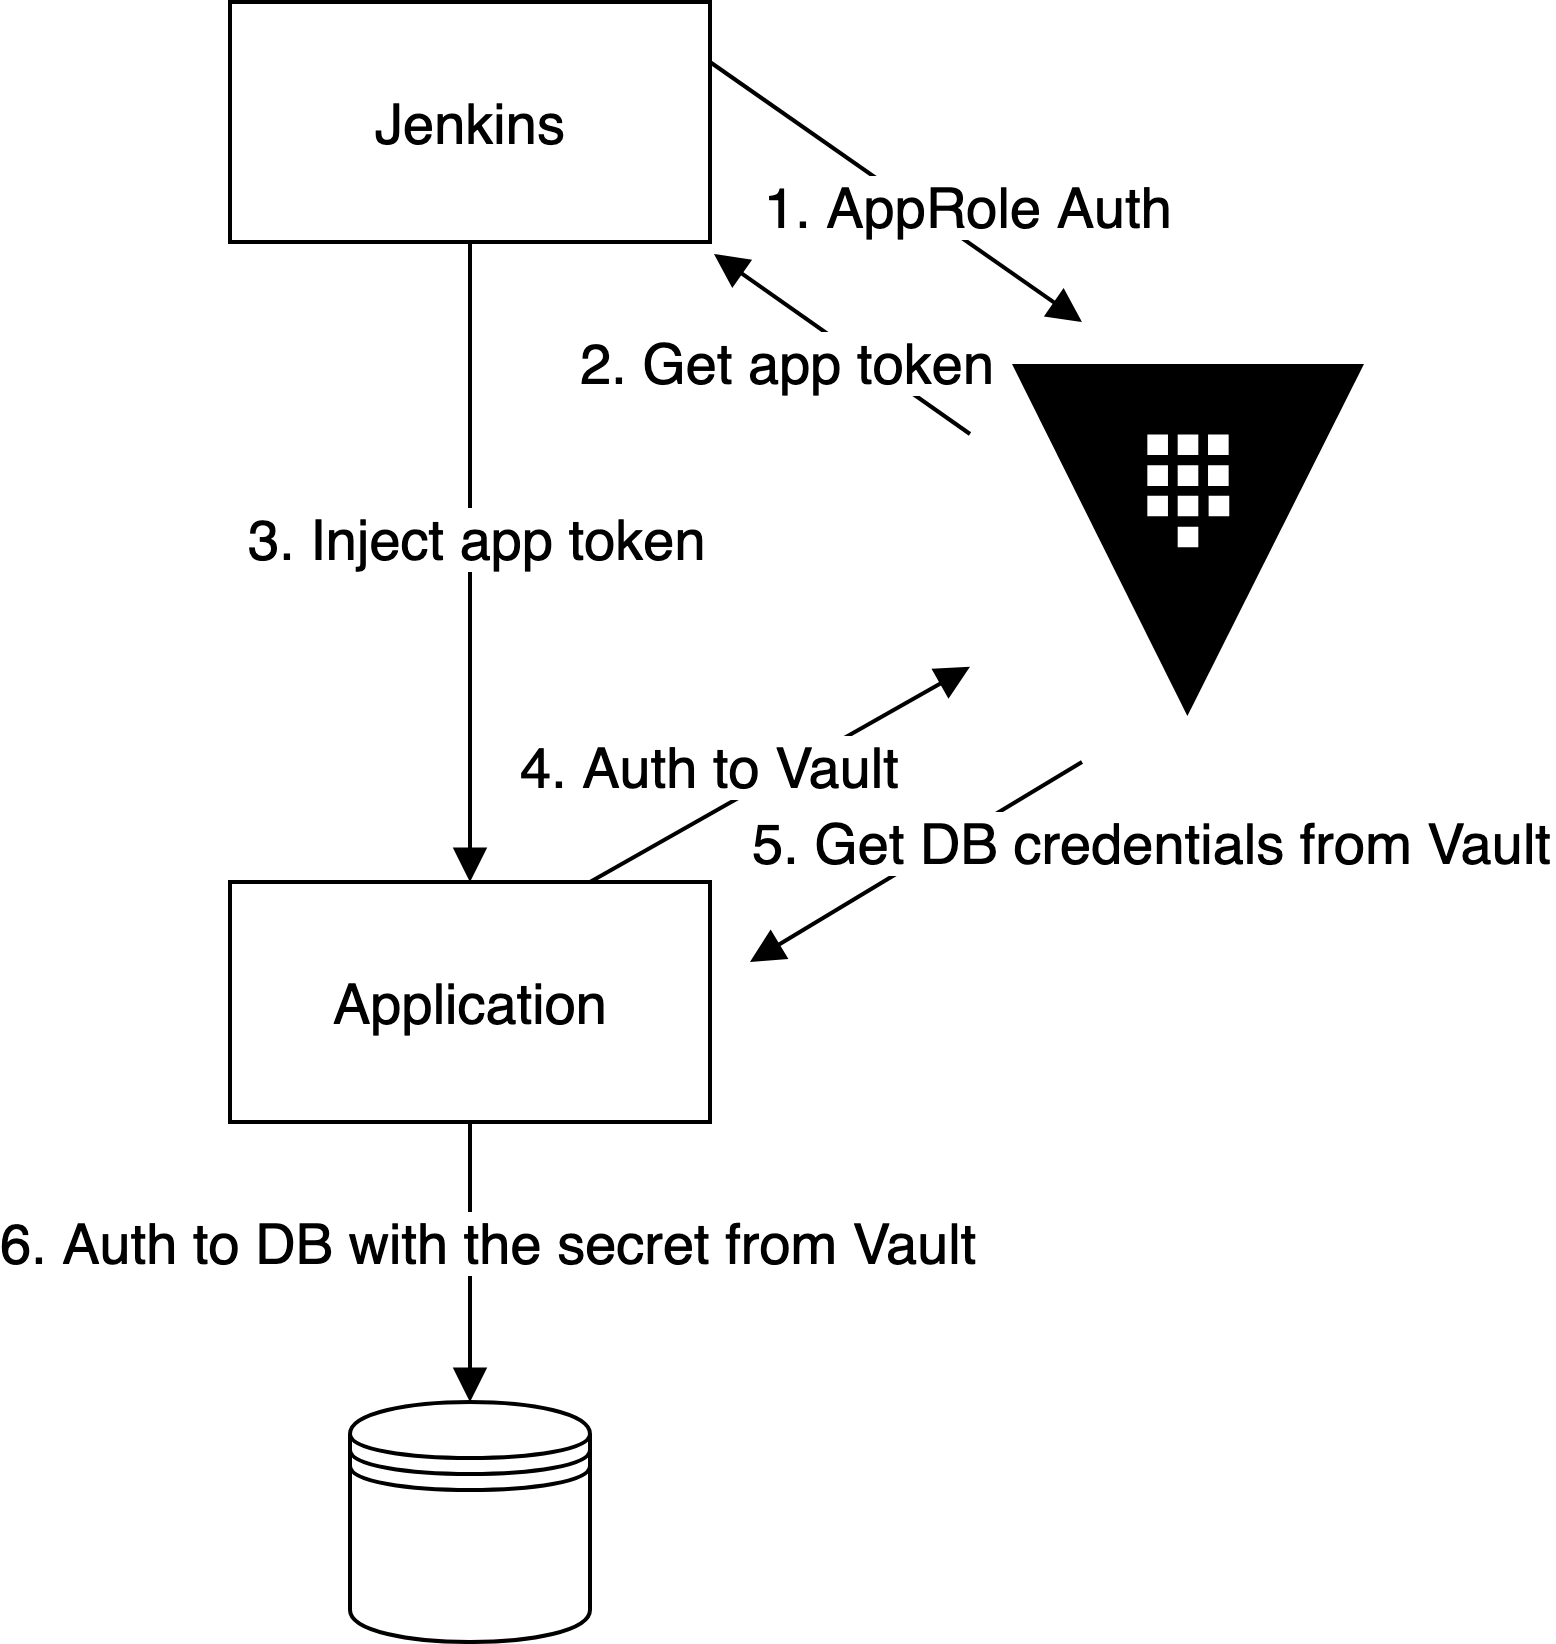
\includegraphics[width=0.6\textwidth]{images/nsip_practical_sec_intro_1.png}
    \caption{Introduction of a secret to its application.}
    \label{practical_sec_intro_1}
\end{figure}

The application is built by a continuous integration (CI) system such as Jenkins: 

\begin{enumerate}
    \setlength\itemsep{1mm}
    \item The CI system authenticates to \textit{Vault}, using AppRole, Role ID, and Secret ID, getting an access token. 
    \item The CI system then generates a new token for the application to use to authenticate to \textit{Vault}. 
    \item The CI system embeds the secret in the application build.
    \item When started, the application uses the embedded token to connect to \textit{Vault}. 
    \item The application can then use the secret, which is the username and password.
    \item Finally, connect to the database.
\end{enumerate}

This process will work, but it has issues. The token is embedded in the application configuration, which directly provides access to the secret. We are  still writing secrets to disk. If the application environment, or container, is compromised, an attacker can take the token straight to \textit{Vault} and retrieve the secret, This is difficult to solve. So how do we deliver a secret to an application without writing it down, persisting it, to accessible storage, such as a disk, or even an environment variable? We can instead use a feature of \textit{Vault} called \textit{response wrapping}, as shown in \autoref{practical_sec_intro_2}.

\begin{figure}
    \centering
    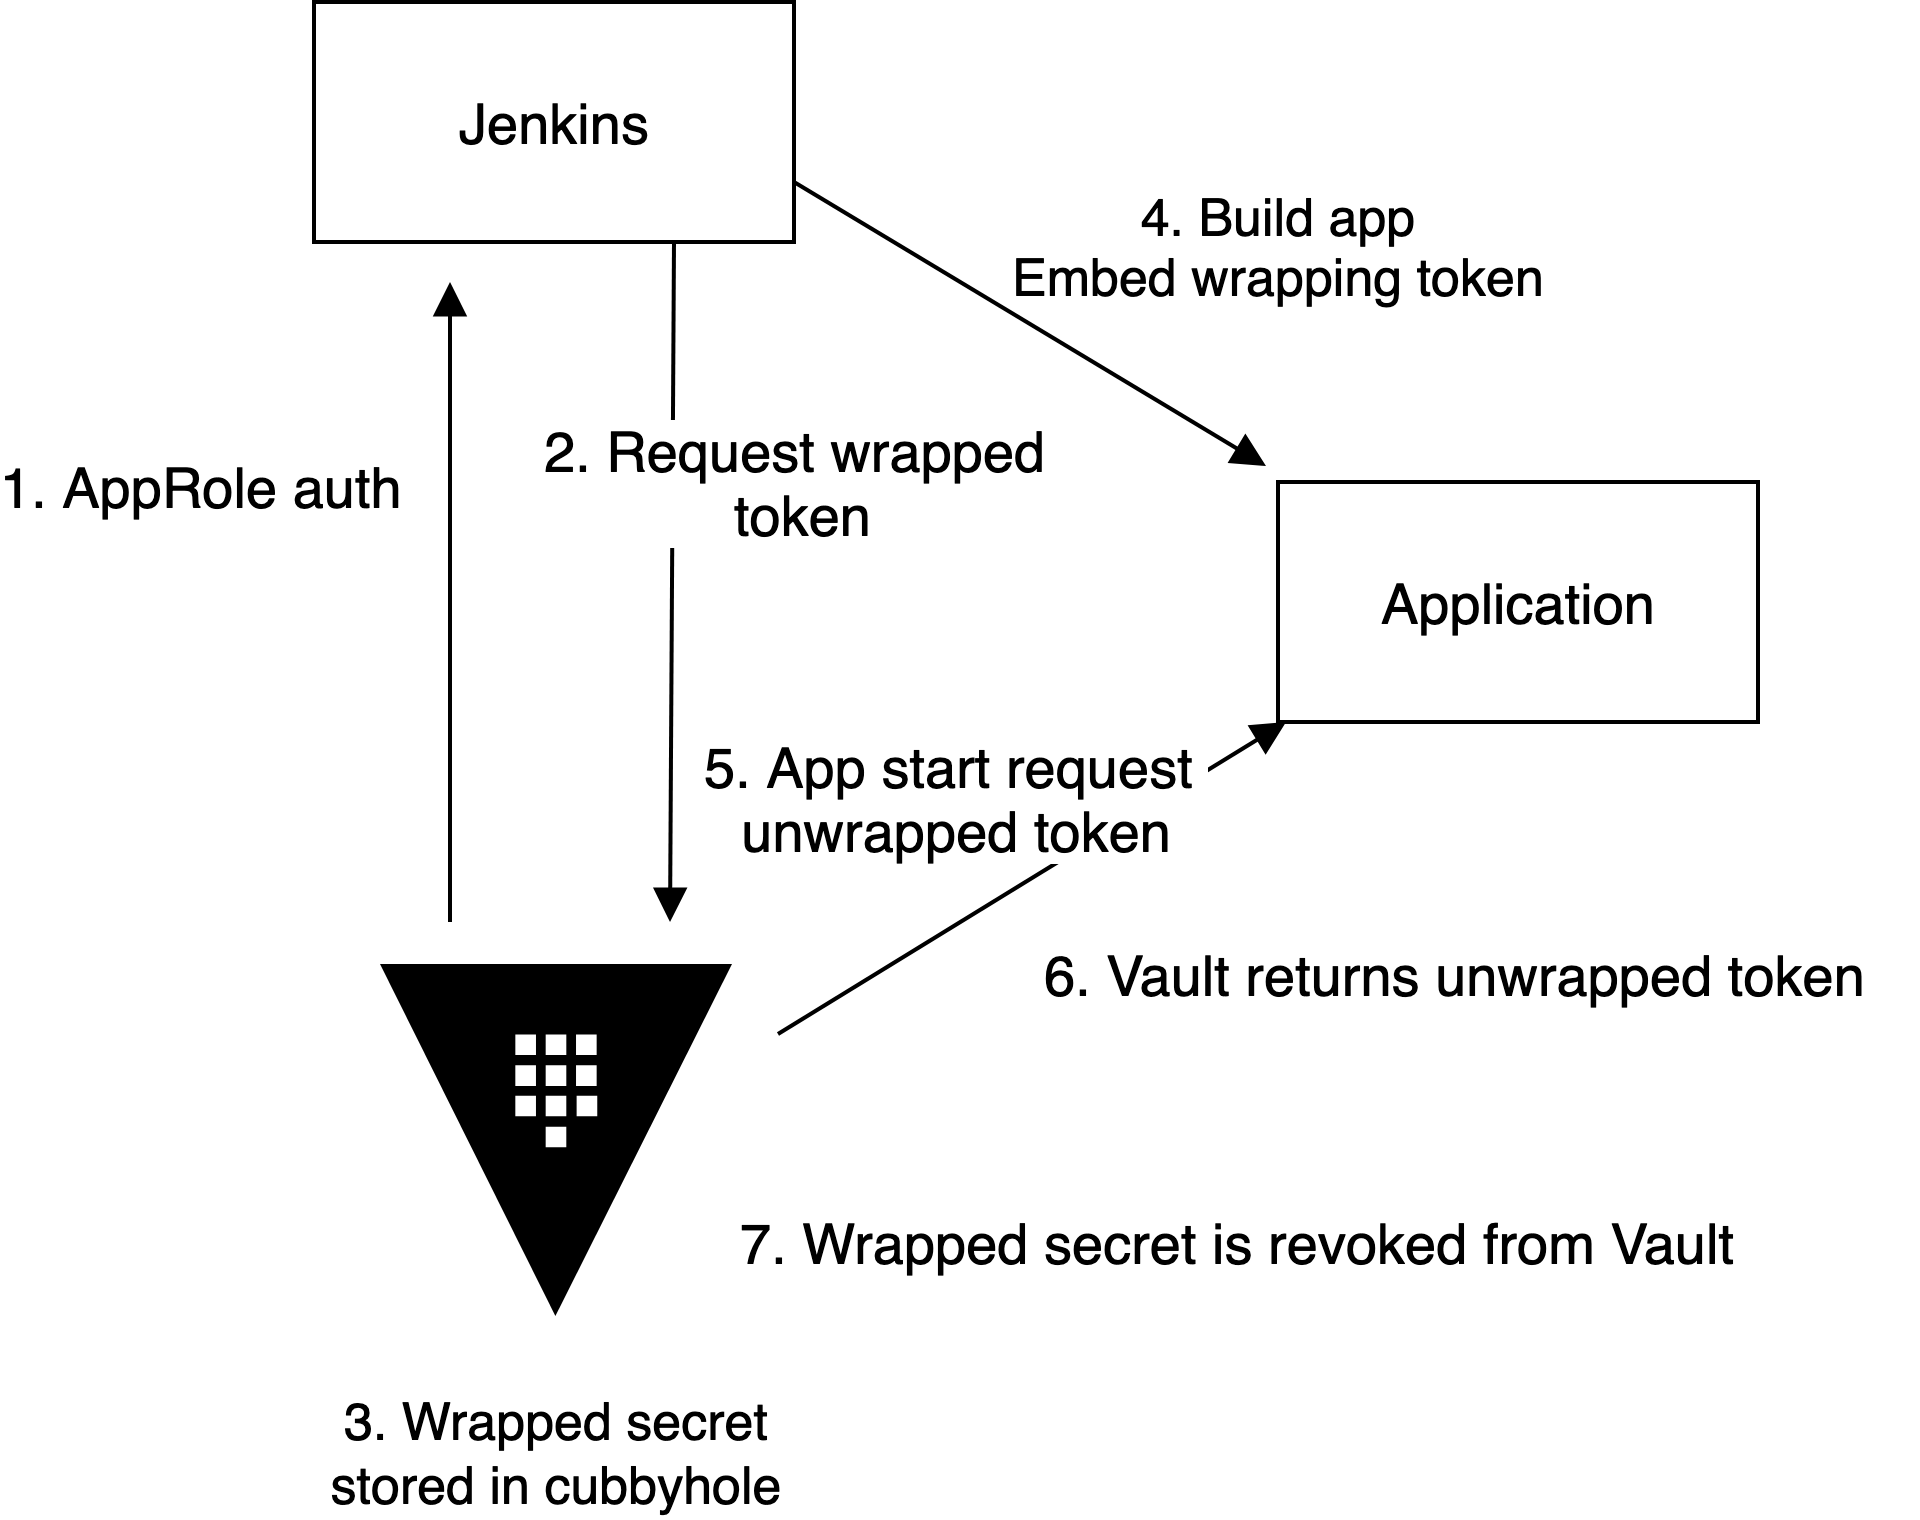
\includegraphics[width=0.6\textwidth]{images/nsip_pracitcal_sec_intro_2.png}
    \caption{Using response wrapping for secret introduction.}
    \label{practical_sec_intro_2}
\end{figure}

\textit{Vault} can generate a wrapped token using the cubbyhole's secret engine. A temporary token, called a wrapping token, is returned to the requester, in this case, Jenkins, and the permanent token is stored in a cubbyhole. Cubbyholes are special KV secrets that are completely revoked when the wrapping token expires. The wrapping token is limited to two uses: once to write the secret, and once more to read it.

The \textit{response wrapping} scenario in \autoref{practical_sec_intro_2} contains the following steps:

\begin{enumerate}
    \setlength\itemsep{1mm}
    \item Using the AppRole authentication method, Jenkis can authenticate against \textit{Vault}.
    \item Jenkins requests a wrapped token instead of a permanent token. 
    \item The permanent token is stored in a cubbyhole.
    \item Jenkins embeds the wrapping token in the application build. 
    \item On startup, the application unwraps the token. 
    \item \textit{Vault} returns the permanent token. 
    \item At this point, the wrapping token is expired, and the permanent token now exists only in the application's memory.
\end{enumerate}

This strategy has a few of advantages: The wrapping token is only valid in the brief window between deployment and application startup. If the wrapping token is stolen after a successful introduction, it's not a problem because it's no longer valid. If the wrapping token is somehow intercepted, the request for the permanent token from the application will fail. If that happens, an alert can be thrown, warning of a potentially compromised secret.

\subsubsection{Integrating Jenkins with Vault -} The first thing we need to do is to install the Jenkins \textit{Vault} plug-in by HashiCorp. The next steps involve \textit{Vault} to enable Jenkins to authenticate: 

\begin{lstlisting}[language=bash]
# Enable secrets engine
$ vault secrets enable -path=secret kv
Success! Enabled the kv secrets engine at: secret/

# Save demo credentials to Vault
$ vault kv put secret/nsip/demo username=dbUser
Success! Data written to: secret/nsip/demo

# Enable the approle authentication method 
$ vault auth enable approle
Success! Enabled approle auth method at: approle/
\end{lstlisting}

The next step is to upload a policy that Jenkins can use to authenticate with approle and to read the secret: 

\begin{lstlisting}[language=bash]
# Login with AppRole
path "auth/approle/login" {
  capabilities = [ "create", "read" ]
}

# Read test data
path "secret/nsip/*" {
  capabilities = [ "read" ]
}
\end{lstlisting}

These two paths give the policy the ability to log in with approle and to read the path in the secrets engine where we saved our secret:

\begin{lstlisting}[language=bash]
# Upload policy to Vault
$ vault policy write jenkins jenkins_policy.hcl
Success! Uploaded policy: jenkins

# Create a authentication role for Jenkins
$ vault write auth/approle/role/jenkins policies=jenkins
Success! Data written to: auth/approle/role/jenkins

# Get role ID for Jenkins analogous to a username
$ vault read auth/approle/role/jenkins/role-id
Key        Value
---        -----
role_id    9ffdab4c-2971-e0f5-039f-1490578cd283

# Get secret ID for Jenkins
$ vault write -f auth/approle/role/jenkins/secret-id
---                   -----
secret_id             fb0d010d-d613-758e-c8c3-8793f768e2ae
secret_id_accessor    39dfceb5-71b0-8193-3a62-986aff2af1ad
\end{lstlisting}

Now we can add these credentials to Jenkins and create a new freestyle project. We enable the \textit{Vault} plugin within the build environment with the following configuration:

\begin{lstlisting}[language=bash]
Vault Url: http://vaultserver:8200
Path: secret/nsip/demo
Environment variable: NSIP_SECRET
Keyname: username
\end{lstlisting}

To demonstrate that Jenkins is able to access the secret, we use a build step: 

\begin{lstlisting}[language=bash]
echo $NSIP_SECRET > secret.txt
\end{lstlisting}

When we build the job, we have the \textit{secret.txt} in our workspace. This was written by the script that we added and we can see our value for our secret written to this file. From here, we can use our imagination, these secrets can be injected into a container. Written to a configuration file, any variety of different mechanisms to inject the secret into an application.

\newpage
% ---- Bibliography ----

\begin{thebibliography}{8}

\bibitem{ref_url_ibm}
IBM - Survey: Most companies use multicloud, but far less have tools for management, \url{https://www.ibm.com/blogs/cloud-computing/2018/10/19/survey-multicloud-management-tools}. Last accessed 20
Mar 2019

\bibitem{ref_url_verizon}
Verizon’s 2018 Data Breach Investigations Report, \url{https://www.verizonenterprise.com/resources/reports/rp_DBIR_2018_Report_en_xg.pdf}. Last accessed 17
Mar 2019

\bibitem{ref_url_guardian}
The Guardian, a Data Breach Overview, \url{https://digitalguardian.com/blog/history-data-breaches}. Last accessed 23
Mar 2019

\bibitem{ref_url_aws}
AWS Secrets Manager, \url{https://aws.amazon.com/secrets-manager}. Last accessed 23
Mar 2019

\bibitem{ref_url_gl}
Kubernetes Secrets Management, \url{https://kubernetes.io/docs/concepts/configuration/secret/}. Last accessed 23
Mar 2019

\bibitem{ref_url_docker}
Docker Swarm Secrets, \url{https://docs.docker.com/engine/swarm/secrets/}. Last accessed 23
Mar 2019

\bibitem{ref_url_vault}
Vault Project, \url{https://www.vaultproject.io}. Last accessed 23
Mar 2019

%\bibitem{se-radio}
%SE-Radio Episode 311: Armon Dadgar on Secrets Management
%\url{http://www.se-radio.net/2017/12/se-radio-episode-311-armon-dadgar-on-secrets-management/}. Last accessed 28 Mar 2019

\bibitem{ref_url_dropbox}
Dropbox, \url{https://www.dropbox.com}. Last accessed 23
Mar 2019

\bibitem{ref_url_owncloud}
ownCloud, \url{https://owncloud.org}. Last accessed 23
Mar 2019

\bibitem{ref_url_1password}
1Pasword, \url{https://1password.com}. Last accessed 23
Mar 2019

\bibitem{ref_url_keepass}
KeePass, \url{https://keepass.info}. Last accessed 23
Mar 2019

\bibitem{ref_url_aws_sms}
AWS Secrets Management Service, \url{https://aws.amazon.com/de/kms/}. Last accessed 23
Mar 2019

\bibitem{vault_vs_chef}
Vault vs. Chef, Puppet, etc., \url{https://www.vaultproject.io/docs/vs/chef-puppet-etc.html}. Last accessed 28
Mar 2019

\bibitem{shamir}
Shamir, A., 1979. How to share a secret. Communications of the ACM, 22(11), pp.612-613.

\bibitem{ref_url_vault_architecture}
Vault Architecture, \url{https://www.vaultproject.io/docs/internals/architecture.html}. Last accessed 19
Mar 2019

\bibitem{aws-kms}
AWS Key Management Service Cryptographic Details
\url{https://d1.awsstatic.com/whitepapers/KMS-Cryptographic-Details.pdf}. Last accessed 28 Mar 2019

\bibitem{aws-sms}
How AWS Secrets Manager Uses AWS KMS
\url{https://docs.aws.amazon.com/kms/latest/developerguide/services-secrets-manager.html}. Last accessed 28 Mar 2019

\bibitem{fips140}
FIPS PUB 140-2
\url{https://csrc.nist.gov/csrc/media/publications/fips/140/2/final/documents/fips1402.pdf}. Last accessed 29 Mar 2019

\bibitem{ref_url_repository}
Practical implementation repository, \url{https://github.com/jmakr0/Secrets-Management}. Last accessed 28
Mar 2019

\end{thebibliography}

\end{document}
